\pgfplotsset{width=1.2\linewidth,height=3.2cm,compat=1.18}
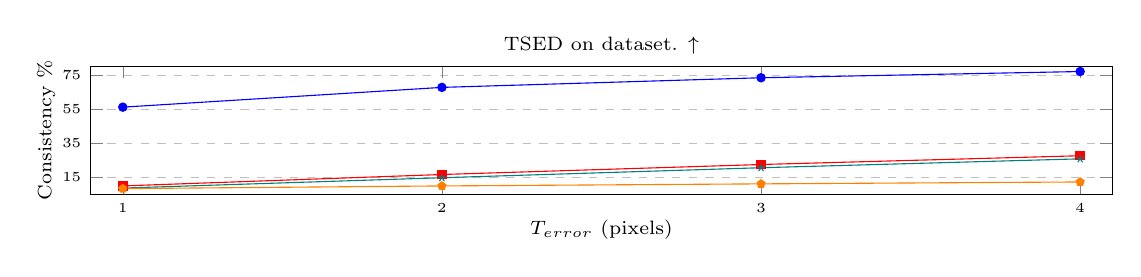
\begin{tikzpicture}
    \begin{axis}[
        title style={align=center, font=\scriptsize, yshift=-.5em},
        title={TSED on dataset. $\uparrow$},
        xlabel={$T_\text{error}$ (pixels)},
        ylabel={Consistency \%},
        xmin=0.9, xmax=4.1,
        ymin=5, ymax=80,
        xtick={1,2,3,4},
        ytick={15,35,55,75},
        legend pos=outer north east,
        legend style={nodes={scale=0.5, transform shape}},
        label style={font=\scriptsize},
        tick label style={font=\tiny},
        ymajorgrids=true,
        grid style=dashed,
        xlabel style={yshift=1ex},
        ylabel style={yshift=-1ex},
        mark size=1.5pt,x
    ]
        \addplot[color=blue,mark=*,] coordinates {
        (1.0,56.1709)(2.0,67.8006)(3.0,73.4705)(4.0,77.1361)
        };
        \addplot[color=red,mark=square*,] coordinates {
        (1.0,9.8101)(2.0,16.5348)(3.0,22.4156)(4.0,27.5712)
        };
        \addplot[color=teal,mark=star,] coordinates {
        (1.0,8.5443)(2.0,14.6361)(3.0,20.5169)(4.0,25.7516)
        }; 
        \addplot[color=orange,mark=pentagon*,] coordinates {
        (1.0,8.2278)(2.0,9.8101)(3.0,11.0232)(4.0,12.1440)
        }; 
    \end{axis}
\end{tikzpicture}
